%=======================02-713 LaTeX template, following the 15-210 template==================
%
% You don't need to use LaTeX or this template, but you must turn your homework in as
% a typeset PDF somehow.
%
% How to use:
%    1. Update your information in section "A" below
%    2. Write your answers in section "B" below. Precede answers for all 
%       parts of a question with the command "\question{n}{desc}" where n is
%       the question number and "desc" is a short, one-line description of 
%       the problem. There is no need to restate the problem.
%    3. If a question has multiple parts, precede the answer to part x with the
%       command "\part{x}".
%    4. If a problem asks you to design an algorithm, use the commands
%       \algorithm, \correctness, \runtime to precede your discussion of the 
%       description of the algorithm, its correctness, and its running time, respectively.
%    5. You can include graphics by using the command \includegraphics{FILENAME}
%
\documentclass[11pt]{article}

\usepackage{amsmath,amssymb,amsthm}
\usepackage{graphicx}
\usepackage[margin=1in]{geometry}
\usepackage{fancyhdr}
\usepackage{comment}
\usepackage{tikz}
\usetikzlibrary{arrows}
\usepackage{caption}
\usepackage{subcaption}


\setlength{\parindent}{0pt}
\setlength{\parskip}{5pt plus 1pt}
\setlength{\headheight}{13.6pt}
\newcommand\question[2]{\vspace{.25in}\hrule\textbf{#1: #2}\vspace{.5em}\hrule\vspace{.10in}}
\renewcommand\part[1]{\vspace{.10in}\textbf{(#1)}}
\newcommand\algorithm{\vspace{.10in}\textbf{Algorithm: }}
\newcommand\correctness{\vspace{.10in}\textbf{Correctness: }}
\newcommand\runtime{\vspace{.10in}\textbf{Running time: }}
\pagestyle{fancyplain}
\lhead{\textbf{\NAME\ \ANDREWID}}
\chead{\textbf{Assignment \HWNUM}}
\rhead{CS 440, Winter 2018}
\begin{document}\raggedright
%Section A==============Change the values below to match your information==================
\newcommand\NAME{Oregon State University}  % your name
\newcommand\ANDREWID{}     % your andrew id
\newcommand\HWNUM{3}              % the homework number
%Section B==============Put your answers to the questions below here=======================

% no need to restate the problem --- the graders know which problem is which,
% but replacing "The First Problem" with a short phrase will help you remember
% which problem this is when you read over your homeworks to study.

The assignment is to be turned in before Midnight (by 11:59pm) on February 1, 2018. 
You should turn in the solutions to the first question as a pdf file through the TEACH website. You should turn in your source code 
for the second question in a single C++ source code file with cpp extension through the TEACH website.

\question{1}{Query processing (3 points)}
Consider the natural join of the relation R and S on attribute A. 
Neither relations have any indexes built on them. 
Assume that R and S have 80000 and 20000 blocks, respectively.
The cost of a join is the number of its block I/Os accesses.

\begin{enumerate}
\item Assume that there are 300 buffer blocks available in the main memory. 
We would like to have the output of join sorted according to attribute A. 
What is the fastest join algorithm for computing the join of R and S? What is the cost of this algorithm? 

\paragraph{solution:} \hfill \break
For this problem I would use standard sort merge Join. I would use this algorithm because it is fairly quick but also because the out put would be in sorted order. Hash merge would actually compute the join more quickly but after we computed the result we would have to sort the results and this would be expensive. Additionally, We can't use the optimized sort merge algorithm because \[ m^2 > B(R) + B(S)\] which in this case is 100,000 which is greater than 90,000.\\

To compute the cost we must first consider the algorithm. The will cost \[ 2 B(R) + 2 B(S)\] in the first pass of the sort. The second pass of the sort similarly will cost \[2 B(R) + 2 B(S) \]. The second pass is also a read and write because we are not just sorting the data. This make writing the data out to the disk after the sort is preformed an intermediate step so we must consider the cost. Finally we must read the data back into the memory to calculate the join. So we can say that the total cost is \[ 5 B(R) + 5 B(s)\]. Given this the cost of this algorithm in this case is \[ 5* (80000 + 20000) \] or 500000 IO operations.\\ 


\item Assume that there are 40 buffer blocks available in the main memory. 
What is the fastest join algorithm to compute the join of R and S? What is the cost of this algorithm? \\

\paragraph{Soution:} \hfill \break
Again we would hope to use Hash merge but given that we only have 40 memory blocks it is not possible to use hash merge. This is because with hash merge you can only have memory squared number of records in one of your relations and \[40^2 < 20,000\]. So for this solution I would again opt to use optimized sort merge.\\

We can Calculate the number of passes and the total cost using the equation shown in the graphic below.\\



Using the equation to compute the number of runs we find that it will take 4 passes to complete the merge sort. This means that the merge costs \[5(B(S) + B(R))\]. However we are not given sorted files so we will need to sort each relation before preforming the merge. This will cos \[2(B(S) + B(R))\]. This means that the total cost of the algorithm is \[7(B(S) + B(R))\]. Given this formula we can say that this will cost \[7 * (80000 + 20000)\] or 700,000 IO operations.\\

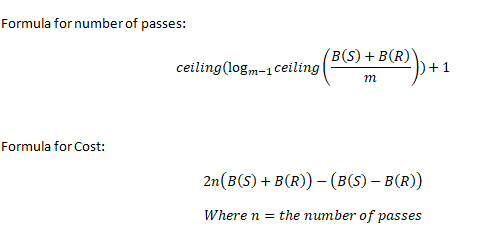
\includegraphics{Formula.PNG}

\item Assume that there are 200 buffer blocks available in the main memory. What is the fastest join 
algorithm to compute the join of R and S? What is the cost of this algorithm? 

\paragraph{Solution:} \hfill \break

In this case we have enough memory to use hash merge. We can do this because \[200^2 > 20000\]. The cost of this algorithm will be \[3 B(R) + 3 B(S)\]. Given this formula we can say that this will cost \[3 * (80000 + 20000)\] or 300000 IO operations.\\

\end{enumerate}



\question{2}{Query processing  (4 points)}
Consider the following relations:
\begin{verbatim}
Dept (did (integer), dname (string), budget (double), managerid (integer))
Emp (eid (integer), ename (string), age (integer), salary (double))
\end{verbatim}

Fields of types \textit{integer}, \textit{double}, and \textit{string} occupy 4, 8, and 40 bytes, respectively. 
Each block can fit at most one tuple of an input relation. There are at most 22 blocks available to the join algorithm in the main memory.
Implement the optimized sort-merge join algorithm for \textit{Dept}~$\bowtie_{Dept.managerid=Emp.eid}$~\textit{Emp} in C++.
\begin{itemize}
\item Each input relation is stored in a separate CSV file, i.e., each tuple is in a separate line and fields of each record are separated by commas.
\item The result of the join must be stored in a new CSV file.
The files that store relations Dept and Emp are Dept.csv and Emp.csv, respectively. 
\item Your program must assume that the input files are in the current working directory, i.e., the one from which your program is running.
\item The program must store the result in a new CSV file with the name join.csv in the current working directory.
\item Your program must run on Linux. Each student has an account on 
\textit{voltdb1.eecs.oregonstate.edu} server, which is a Linux machine. You may use this machine to test your program if you do not have access to any other Linux machine. You can use the following \textit{bash} command to connect to \textit{voltdb1}:
\begin{verbatim}
> ssh your_onid_username@voltdb1.eecs.oregonstate.edu
\end{verbatim}
Then it asks for your ONID password and probably one another question. You can only access this server on campus.

\item You can use following commands to compile and run C++ code:

\begin{verbatim}
> g++ main.cpp -o main.out
> main.out
\end{verbatim}

\end{itemize}

\end{document}
